Niezależnie od tego, czy posiadasz płytę główną z BIOS-em, czy z UEFI, w poprzednim punkcie powinieneś wybrać \textcolor{ubuntu_orange}{Zainstaluj Ubuntu}. Ta metoda jest szybsza od \textcolor{ubuntu_orange}{Wypróbuj Ubuntu bez instalowania}, gdyż nie wymaga załadowania całego systemu. Jeżeli mimo wszystko uruchomiłeś cały system w trybie Live, to na pulpicie znajdziesz ikonę \textcolor{ubuntu_orange}{Zainstaluj Ubuntu} (lub ,,Install Ubuntu'', jeżeli nie zmieniałeś języka). Od tego momentu instalacja przebiega w identyczny sposób dla każdego wybranego sposobu instalacji.

W czasie instalacji w prawej części paska u góry ekranu znajduje się szereg ikon:
\begin{description}
\item[
\includegraphics{images/ikony_dostempnosc.png}]\textcolor{ubuntu_orange}{Dostępność} --- uruchomienie lupy, czytnika ekranowego lub klawiatury ekranowej;
\item[
\includegraphics{images/ikony_internet.png}]\textcolor{ubuntu_orange}{Łączność} --- konfiguracja połączenia z internetem na czas instalacji systemu;
\item[
\includegraphics{images/ikony_jezyk.png}]\textcolor{ubuntu_orange}{Język} --- zmiana języka oraz układu klawiatury na czas instalacji systemu;
\item[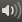
\includegraphics{images/ikony_dzwiek.png}]\textcolor{ubuntu_orange}{Ustawienia głośności i dźwięku};
\item[
\includegraphics{images/ikony_zasilanie.png}]\textcolor{ubuntu_orange}{Zasilanie} --- wyłączenie lub ponowne uruchomienie komputera.
\end{description}
\clearpage
\subsubsection{Wybór języka}
\begin{center}
        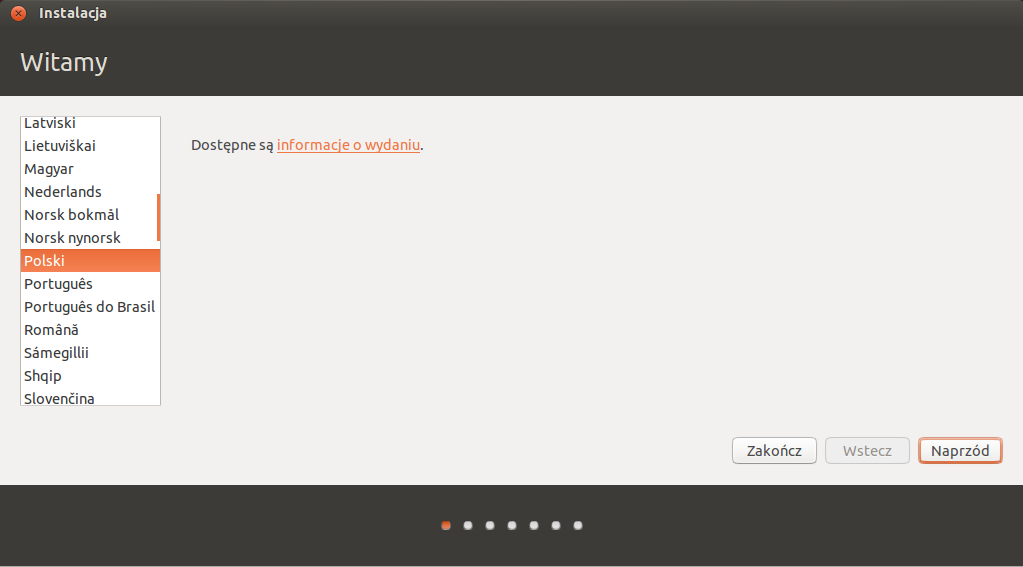
\includegraphics[width=\linewidth]{images/instalator_jezyk.png}
\end{center}

Pierwszy ekran instalatora pozwala wybrać język. Jeżeli wcześniej nie zmieniłeś języka na polski, to teraz masz ku temu okazję. Język wybrany podczas instalacji będzie także domyślnym językiem zainstalowanym w systemie.
\begin{flushright}
Kliknij przycisk \textcolor{ubuntu_orange}{Naprzód}, aby przejść dalej.
\end{flushright}
\clearpage
\subsubsection{Konfiguracja Wi-Fi}
\begin{center}
        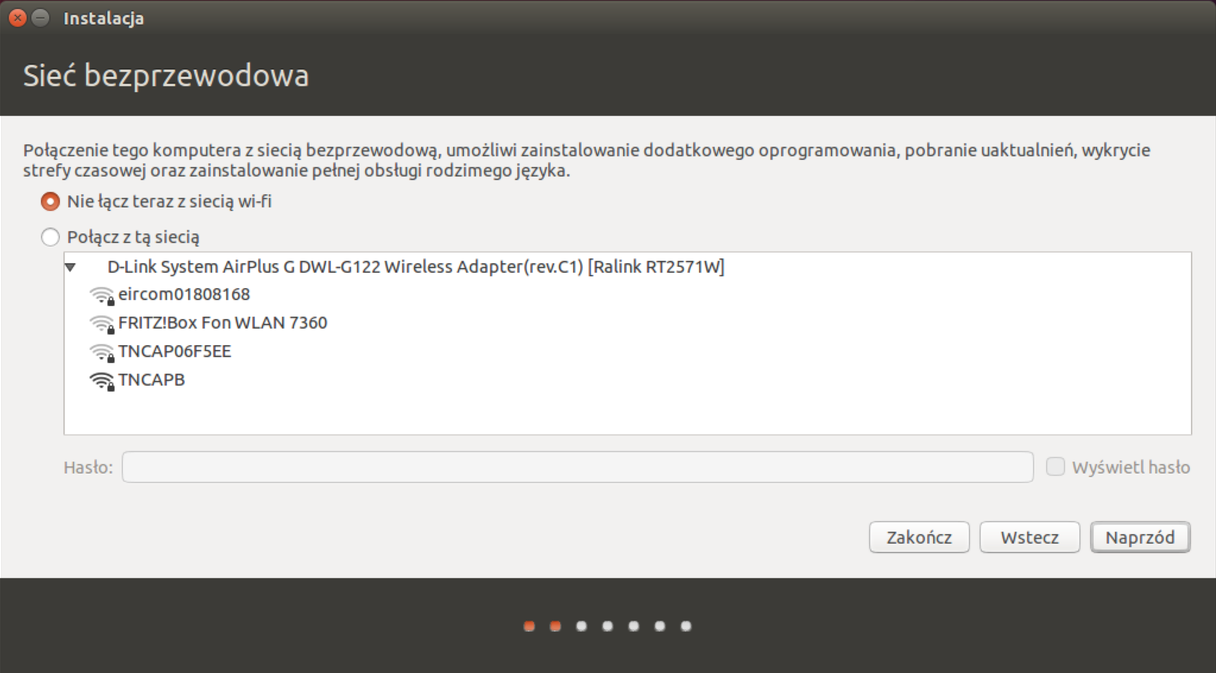
\includegraphics[width=\linewidth]{images/instalator_wifi.png}
\end{center}

Drugi ekran instalatora pozwala skonfigurować połączenie bezprzewodowe Wi-Fi. Jeżeli instalator nie wykryje żadnej karty Wi-Fi, to nie pokaże tego ekranu. Ten etap instalacji zostanie pominięty również wtedy, gdy uda się nawiązać połączenie przewodowe.

Z listy na ekranie wybierz sieć bezprzewodową, z którą chcesz się połączyć. Wpisz hasło do sieci bezprzewodowej w pole \textcolor{ubuntu_orange}{Hasło}.
\begin{flushright}
Kliknij przycisk \textcolor{ubuntu_orange}{Naprzód}, aby przejść dalej.
\end{flushright}
\clearpage
\subsubsection{Sprawdzenie kompatybilności sprzętu, wybór dodatkowych komponentów}
\begin{center}
        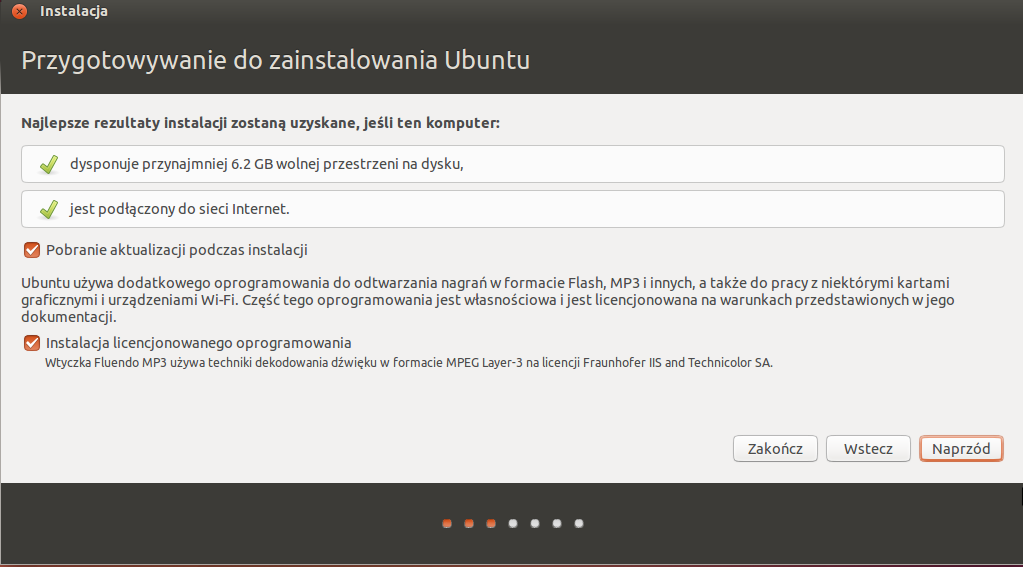
\includegraphics[width=\linewidth]{images/instalator_wymagania.png}
\end{center}

Na tym etapie instalator sprawdzi, czy na dysku twardym jest wystarczająco dużo miejsca, aby zainstalować Ubuntu. Połączenie z internetem nie jest wymagane do zainstalowania systemu, jest jednak niezbędne, by zainstalować spolszczenie, aktualizacje oraz dodatkowe wtyczki. Jeżeli w tym momencie nie masz połączenia z internetem, to pobranie paczek lokalizacyjnych będzie możliwe później. Zostało to opisane w rozdziale \ref{rzeczy_do_zrobienia_po_instalacji} ,,Rzeczy do zrobienia po instalacji Ubuntu''.
\begin{itemize}
\item \textcolor{ubuntu_orange}{Pobieranie aktualizacji podczas instalacji} --- instalator pobierze i zainstaluje wszystkie aktualizacje, które zostały wydane od dnia premiery systemu.
\item \textcolor{ubuntu_orange}{Instalacja licencjonowanego oprogramowania} --- w skład pakietu wchodzą własnościowe sterowniki do kart graficznych AMD lub Nvidii, sterowniki do kart Wi-Fi, kodeki audio-wideo (po instalacji Ubuntu będzie w stanie odtworzyć prawie każdy rodzaj plików muzycznych i filmowych) oraz wtyczka Flash do przeglądarki internetowej.
\end{itemize}
\begin{flushright}
Kliknij przycisk \textcolor{ubuntu_orange}{Naprzód}, aby przejść dalej.
\end{flushright}
\clearpage
\subsubsection{Partycjonowanie dysku twardego}
\begin{center}
        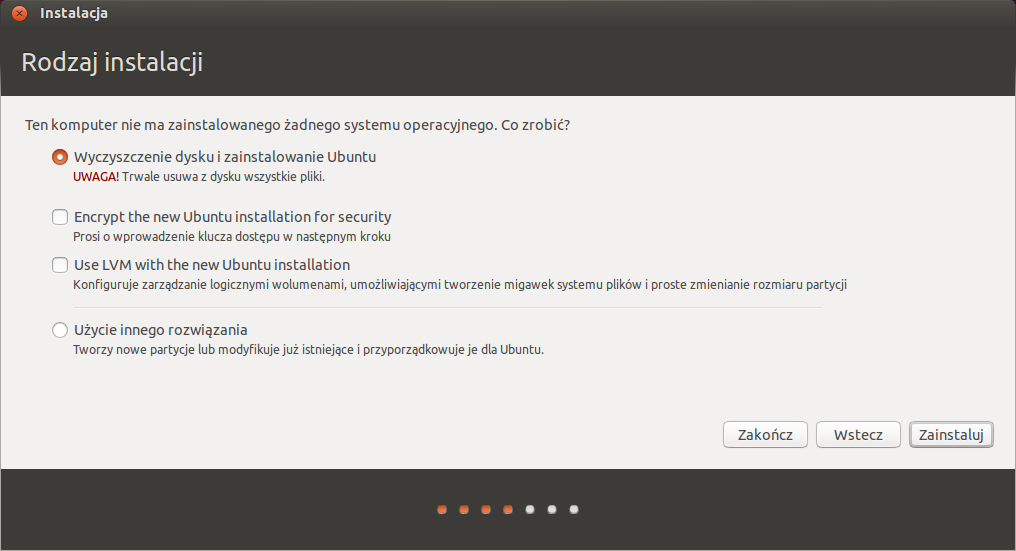
\includegraphics[width=\linewidth]{images/instalator_partycjonowanie_proste.png}
\end{center}

Jest to najważniejszy etap instalacji. W tym miejscu można dokonać cudów, jak i zniszczyć cały dysk twardy. Jako że prawidłowe partycjonowanie dysku twardego to bardzo szeroki temat, poświęciliśmy mu cały osobny rozdział. Na powyższym obrazie widać najprostszą wersję tego etapu instalacji. Na dysku twardym nie ma zainstalowanego żadnego systemu operacyjnego i instalator proponuje wykorzystanie całej przestrzeni dla Ubuntu. Jeżeli masz inne systemy operacyjne, to instalator zaproponuje wydzielenie miejsca i instalację Ubuntu obok danego systemu operacyjnego. Jeżeli miałeś wcześniej zainstalowane Ubuntu, instalator zaproponuje aktualizację do najnowszego wydania lub usunięcie i zainstalowanie Ubuntu ponownie.
Partycjonowanie zostało szeroko opisane w rozdziale \ref{subsec:partycjonowanie} ,,Zaawansowane partycjonowanie''. Wróć tutaj, gdy go przeczytasz.
\begin{flushright}
Kliknij przycisk \textcolor{ubuntu_orange}{Naprzód}, aby przejść dalej.
\end{flushright}
\clearpage
\subsubsection{Wybór strefy czasowej}
\label{instalator_strefa_czasowa}
\begin{center}
        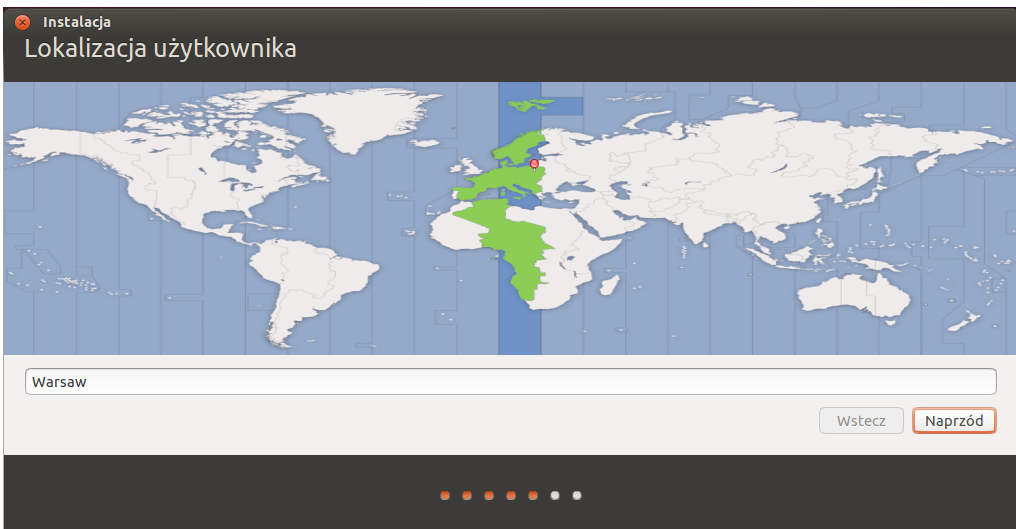
\includegraphics[width=\linewidth]{images/instalator_czas.png}
\end{center}

Na tym etapie należy wybrać lokalizację tego komputera, aby system mógł wyświetlać prawidłowy czas i automatycznie dostosowywać się do zmian pomiędzy czasem letnim i zimowym. Jeżeli w trakcie instalacji masz połączenie z internetem, to odpowiednia lokalizacja zostanie wybrana automatycznie. Jeżeli nie masz dostępu do internetu, w pole wpisz \textcolor{ubuntu_orange}{Warsaw}. Stolica naszego kraju określa też naszą strefę czasową.
\begin{flushright}
Kliknij przycisk \textcolor{ubuntu_orange}{Naprzód}, aby przejść dalej.
\end{flushright}
\clearpage
\subsubsection{Wybór układu klawiatury}
\begin{center}
        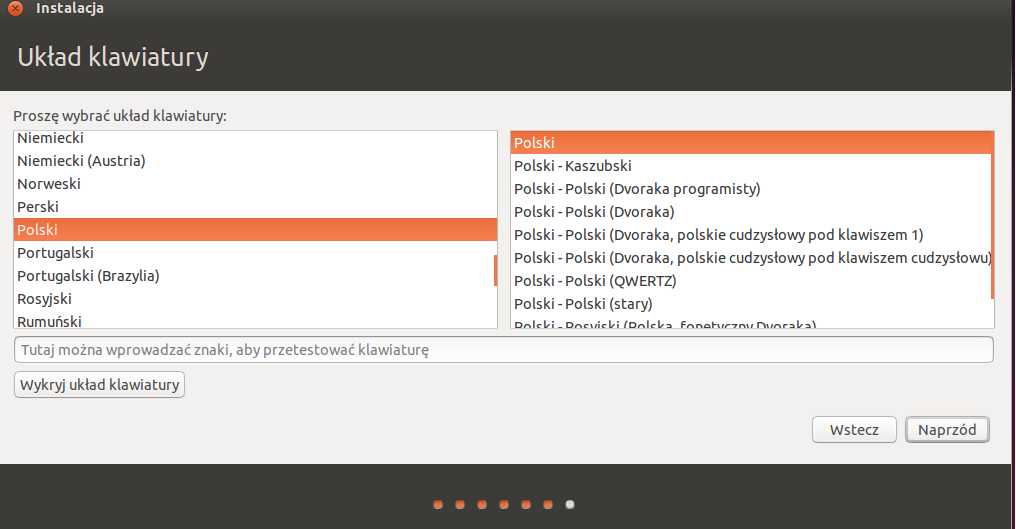
\includegraphics[width=\linewidth]{images/instalator_klawiatura.png}
\end{center}

Ten ekran pozwala wybrać układ klawiatury. Jeżeli wybrałeś wcześniej język polski, to standardowa polska klawiatura zostanie wybrana automatycznie. W polu możesz wpisać kilka znaków, aby sprawdzić, czy zaznaczony układ odpowiada rzeczywistości. Pierwsza opcja (\textcolor{ubuntu_orange}{Polski}) to standardowa klawiatura mieszcząca 101 klawiszy, zwana potocznie układem programisty.
Nie zalecamy korzystania z funkcji \textcolor{ubuntu_orange}{Wykryj układ klawiatury}. Korzystając ze wskazówek instalatora otrzymamy klawiaturę amerykańską, nieobsługującą polskich znaków diakrytycznych.
\begin{flushright}
Kliknij przycisk \textcolor{ubuntu_orange}{Naprzód}, aby przejść dalej.
\end{flushright}
\clearpage
\subsubsection{Tożsamość użytkownika}
\begin{center}
        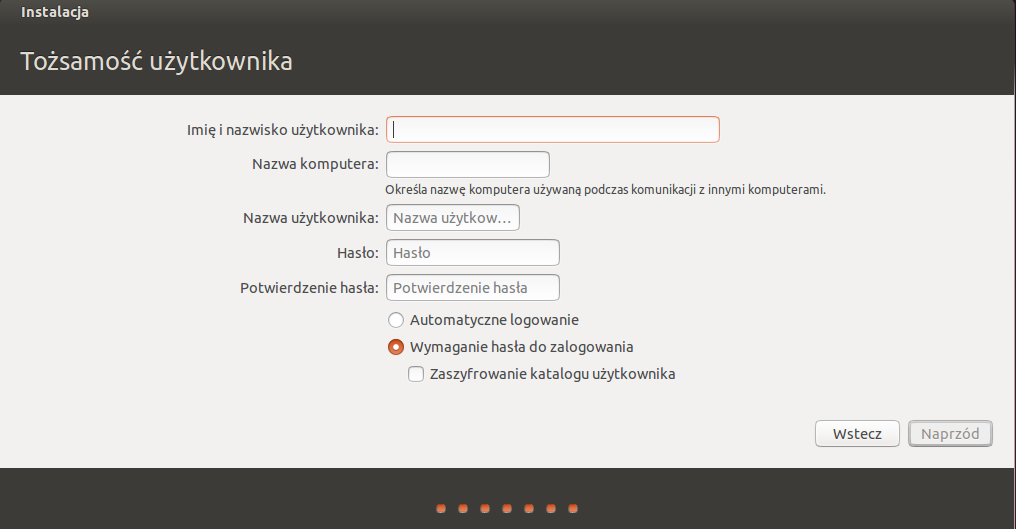
\includegraphics[width=\linewidth]{images/instalator_dane.png}
\end{center}

To już ostatni etap instalacji. Te pola należy uzupełnić, aby system mógł cię prawidłowo zidentyfikować.
\begin{itemize}
\item \textcolor{ubuntu_orange}{Imię i nazwisko użytkownika} --- pole nieobowiązkowe, ale jeżeli uzupełnisz te dane, to system będzie się do ciebie zwracał imieniem i nazwiskiem, zamiast używać loginu (np. Jan Kowalski).
\item \textcolor{ubuntu_orange}{Nazwa komputera} --- określa, jak będzie się nazywał twój komputer (np. laptop).
\item \textcolor{ubuntu_orange}{Nazwa użytkownika} --- twój login do systemu (np. jan\_kowalski, albo twój pseudonim). Login nie może zawierać wielkich liter, spacji, ani znaków specjalnych.
\item \textcolor{ubuntu_orange}{Hasło} --- hasło do komputera. Hasło zabezpiecza system przed nieuprawnionym dostępem.\\
Uwaga: Ustawienie hasła uniemożliwia innym zalogowanie się do twojego konta, jednak nie zabezpiecza przed podejrzeniem przez inne osoby twoich danych, o ile ich nie zaszyfrujesz. 
\item \textcolor{ubuntu_orange}{Potwierdzenie hasła} --- wpisz ponownie to samo hasło, co w polu powyżej.
\item \textcolor{ubuntu_orange}{Automatyczne logowanie} --- jeżeli zaznaczysz to pole, system automatycznie zaloguje tego użytkownika po uruchomieniu. Nie będzie potrzebne podawanie hasła, aby uzyskać dostęp do komputera.
\item \textcolor{ubuntu_orange}{Wymaganie hasła do zalogowania} --- po uruchomieniu komputera będziesz musiał podać hasło, aby uzyskać dostęp do swojego konta.
\item \textcolor{ubuntu_orange}{Zaszyfrowanie katalogu użytkownika} --- jeżeli zaznaczysz to pole, twoje prywatne dane zostaną zaszyfrowane. Nikt nieznający hasła nie będzie mógł uzyskać dostępu do twoich plików. Jeżeli zapomnisz hasło, to bezpowrotnie utracisz dostęp do swoich plików.
\end{itemize}
\begin{flushright}
Kliknij przycisk \textcolor{ubuntu_orange}{Naprzód}, aby przejść dalej.
\end{flushright}
\clearpage
\subsubsection{Instalacja}
\begin{center}
        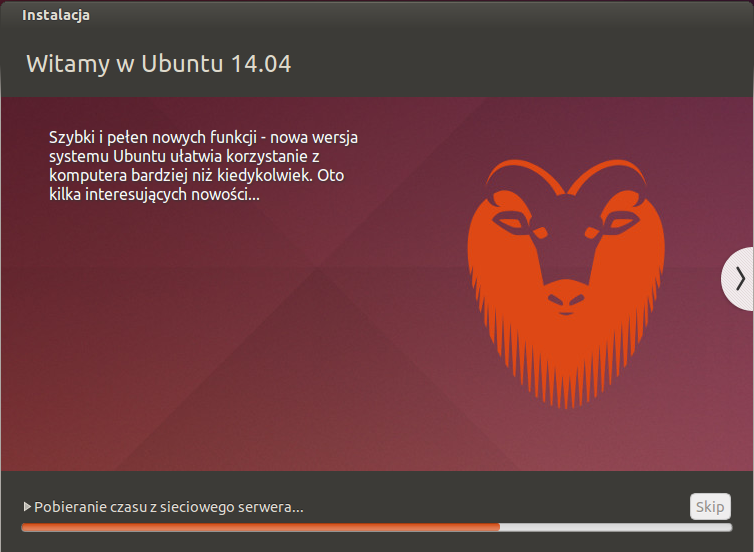
\includegraphics[width=\linewidth]{images/instalator_kopiowanie.png}
\end{center}

Teraz system dokona instalacji na dysku twardym oraz ewentualnie pobierze i zainstaluje paczki językowe, aktualizacje i dodatkowe oprogramowanie. Proces ten może potrwać od kilku do kilkunastu minut, w zależności od klasy komputera, ilości zadań do wykonania oraz szybkości łącza internetowego. Po zakończeniu instalacji zostaniesz poproszony o usunięcie nośnika instalacyjnego i ponowne uruchomienie komputera. Jeżeli wszystko poszło pomyślnie, to za minutę zostaniesz przywitany pulpitem Ubuntu.
\begin{flushright}
\textcolor{ubuntu_orange}{Gratulacje!} Właśnie zainstalowałeś Ubuntu 14.04 LTS Trusty Tahr.\\
Komputer zostanie zresetowany.\\
Przejdź do sekcji \ref{pierwsze_uruchomienie}:,,Pierwsze uruchomienie Ubuntu''.
\end{flushright}
\clearpage
